\usetikzlibrary{arrows.meta,calc}
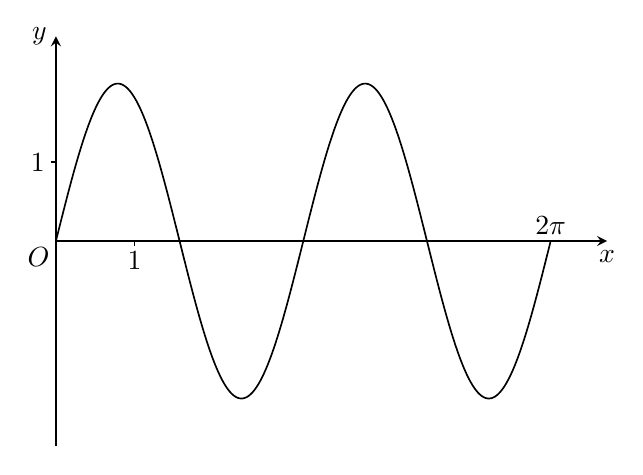
\begin{tikzpicture}[x=1cm,y=1cm,line width=.6pt,>=stealth]
\draw[->] (0,0)--(7.0,0);
\node[below,inner sep=0pt,yshift=-3pt] at (7.0,0) {$x$};
\draw[->] (0,-2.6)--(0,2.6);
\node[left,inner sep=0pt,xshift=-3pt] at (0,2.6) {$y$};
\node[below left,inner sep=0pt,xshift=-2pt,yshift=-2pt] at (0,0) {$O$};
\draw (0,1)--(-0.06,1);
\node[left,inner sep=0pt,xshift=-2pt] at (-0.06,1) {$1$};
\draw (1,0)--(1,-0.06);
\node[below,inner sep=0pt,yshift=-2pt] at (1,-0.06) {$1$};
\draw[domain=0:6.2831853,samples=260] plot (\x,{2*sin(deg(2*\x))});
\node[above,inner sep=0pt,yshift=2pt] at (6.2831853,0) {$2\pi$};
\end{tikzpicture}
